


\begin{figure}
  \centering
  \begin{subfigure}{0.48\textwidth}
    \centering
    \includegraphics[width=\textwidth]{Pics/threshold_no_lase.jpg}
    \caption{The voltage is below the lasing threshold.}
    \label{fig:no_lase}
  \end{subfigure}
  \begin{subfigure}{0.48\textwidth}
    \centering
    \includegraphics[width=\textwidth]{Pics/threshold_lase.jpg}
    \caption{The voltage is above the lasing threshold.}
    \label{fig:lase}
  \end{subfigure}
\end{figure}


\begin{figure}
  \centering
  \includegraphics[width=0.5\textwidth]{Pics/Rb_florescence.jpg}
  \caption{Rubidium florescense line.}
  \label{fig:florescence}
\end{figure}

\begin{figure}
  \centering
  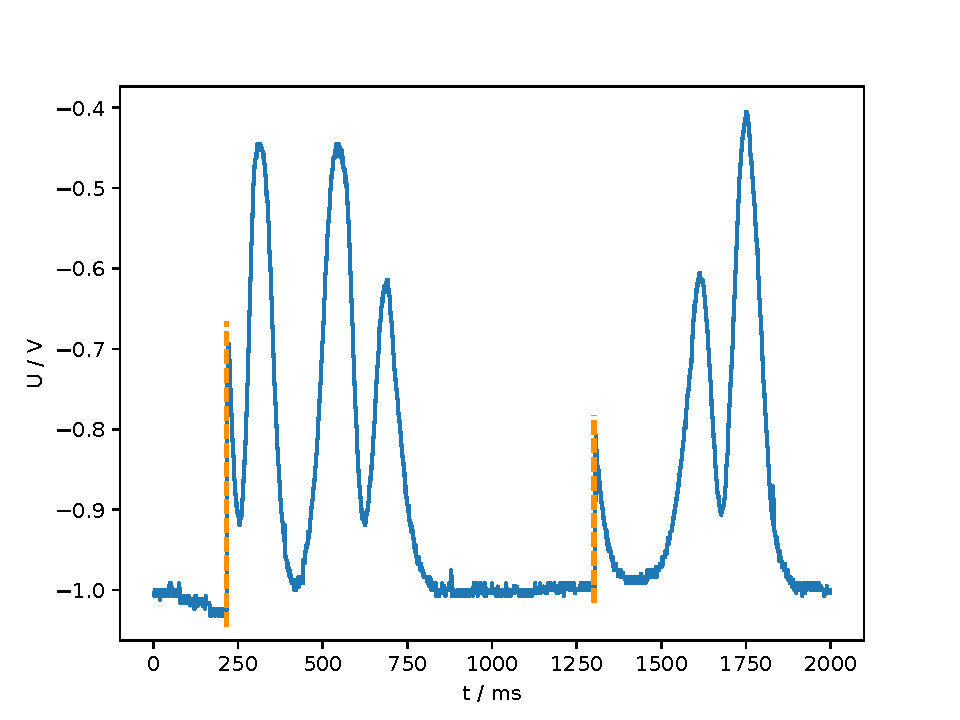
\includegraphics[width=0.7\textwidth]{Pics/example_spectrum_hop.pdf}
  \caption{Example spectrum. The mode hopes are indicated by the orange markers.}
  \label{fig:example}
\end{figure}

\begin{figure}
  \centering
  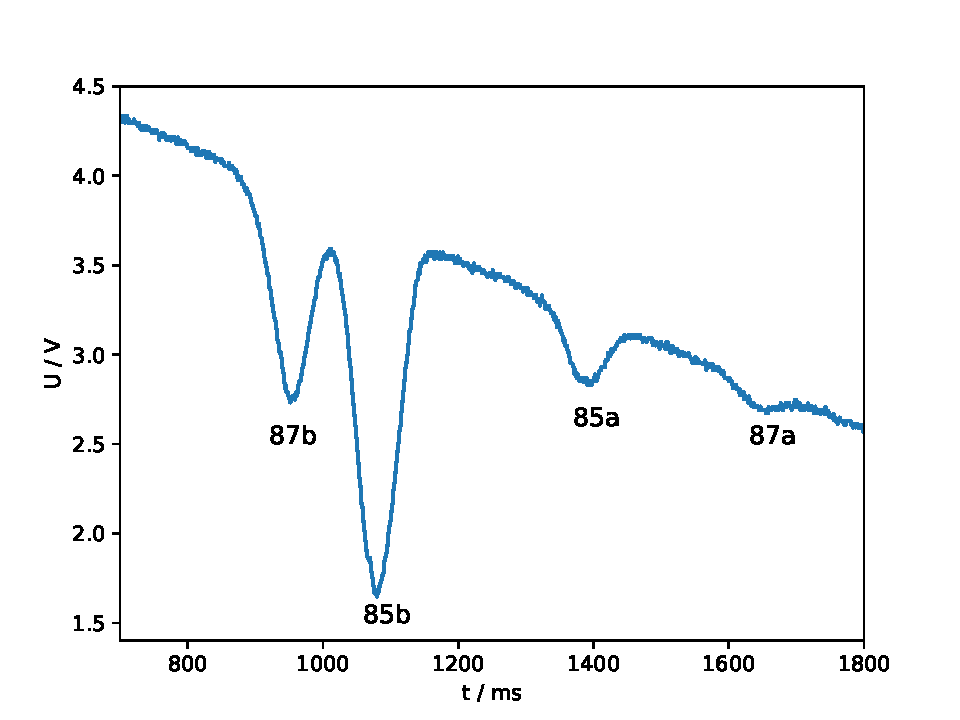
\includegraphics[width=0.7\textwidth]{Pics/Rb_spectrum.pdf}
  \caption{Rubidium spectrum.}
  \label{fig:spectrum}
\end{figure}

\begin{figure}
  \centering
  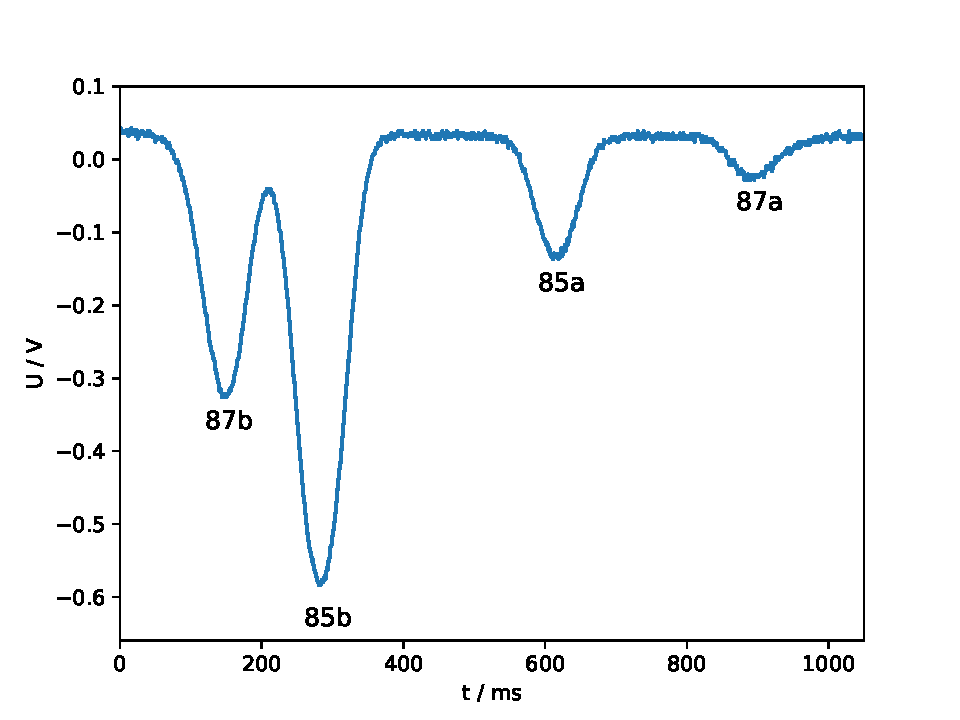
\includegraphics[width=0.7\textwidth]{Pics/Rb_spectrum_subst.pdf}
  \caption{Rubidium spectrum with substraction technique.}
  \label{fig:spectrum_sub}
\end{figure}
